\begin{frame}
	\frametitle{Linear mixed effects models}
	
	\begin{itemize}
		\item Extension of linear regression
		\item Take into account within and between groups variance
		\item ``Mixed'': Fixed + random factors
		\item Fixed: systematic effect
		\item Random: non-systematic sources of variance; e.g.~some participants are faster than others
		\item $lmer()$; part of $lme4$ \cite{bates2015}
	\end{itemize}

\end{frame}


\begin{frame}[fragile]
	\frametitle{Linear mixed effects models}

\begin{minipage}{.6\textwidth}
	\begin{itemize}
		\item New simulated data frame.
		\item Uncover known parameter $\beta = 50$
		\item Added by-subjects variance:
		\item[] By-subjects intercepts and slopes.
		\item Models $LM\_observations\_in\_subj.R$	
		\item What do you observe?			
		\item What's the evidence that this parameter is different from 0 (i.e. null hypothesis)?
%		\item Task 1/2: Fit $lm()$s
%		\item Task 3: Fit two $lmer()$s models on data using random effects structure
	\end{itemize}
\end{minipage}	
\hfill
\begin{minipage}{.35\textwidth}
	\begin{verbatim}
> head(data)
	subj cond         y
   1    a  71.05932
   1    a  62.23969
   1    a  63.93085
   1    a  57.07717
   1    a  56.54501
   1    a  70.29821
	\end{verbatim}
\end{minipage}	
	
		%\texttt{m <- lmer(outcome variance $\sim$ predictor + random effect, data frame)}
\end{frame}



\begin{frame}[fragile]
	\frametitle{Linear mixed effects models}

%	\begin{minipage}{1\textwidth}
		\uncover<1->{\texttt{> m1 <- lm(y $\sim$ cond, data)}\\}
		\uncover<2->{\texttt{> m2 <- lm(ysubjmeans $\sim$ cond, data.subj)}\\}
		\uncover<3->{\texttt{> m3a <- lmer(y $\sim$ cond + (1|subj), data)}\\}
		\uncover<4->{\texttt{> m3b <- lmer(y $\sim$ cond + (1+cond|subj), data)}\\}
%	\end{minipage}
%	\begin{minipage}{\textwidth}
	\begin{table}[!htbp] \centering 
		\caption{Estimates (see $models\_random\_effects.R$)} 
		\begin{tabular}{@{\extracolsep{5pt}} ccccc} 
			\\[-1.8ex]\hline 
			& Estimate & Std. Error & t value & Pr(\textgreater \textbar t\textbar ) \\ 
			\hline \\[-1.8ex] 
			\texttt{m1} &  $51.189$ & $1.169$ & $43.784$ & $< 0.001$ \\ 
			\uncover<2->{\texttt{m2} & $51.189$ & $2.823$ & $18.135$ & $< 0.001$} \\
			\uncover<3->{\texttt{m3a} &  $51.189$ & $0.860$ & $59.506$ & \only<5>{?} }\\ 
			\uncover<4->{\texttt{m3b} & $51.189$ & $1.506$ & $33.989$ & \only<5>{?} }\\ 
			\hline \\[-1.8ex] 
		\end{tabular} 
	\end{table} 
%    \end{minipage}
	
%	\begin{minipage}{.5\textwidth}			
%	\begin{verbatim}


	
%	\end{verbatim}
 %   \end{minipage}	
	
\end{frame}


\begin{frame}
	\frametitle{Linear mixed effects models}
	
	\begin{figure}
		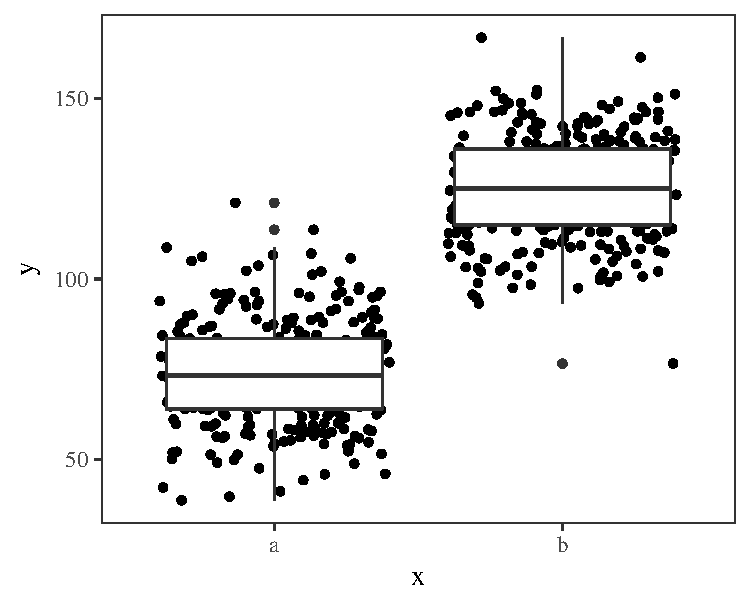
\includegraphics[scale = .6]{gfx/rawdata.pdf}
		\caption{Simulated data}
	\end{figure}
	
\end{frame}


\begin{frame}
	\frametitle{Linear mixed effects models}
	
	\begin{figure}
		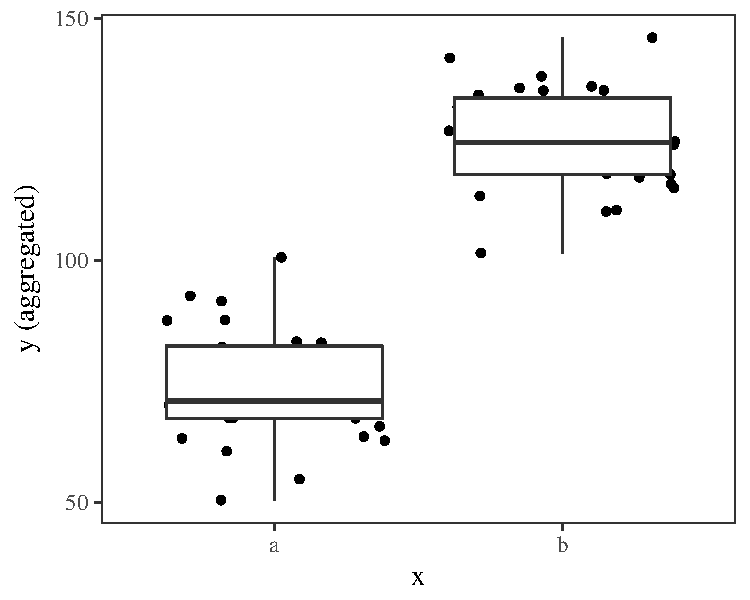
\includegraphics[scale = .6]{gfx/aggregateddata.pdf}
		\caption{Simulated data, aggregated by subject and condition}
		\end{figure}
		
\end{frame}

%\begin{frame}
%	\frametitle{Linear mixed effects models}
%	
%	\begin{figure}
%		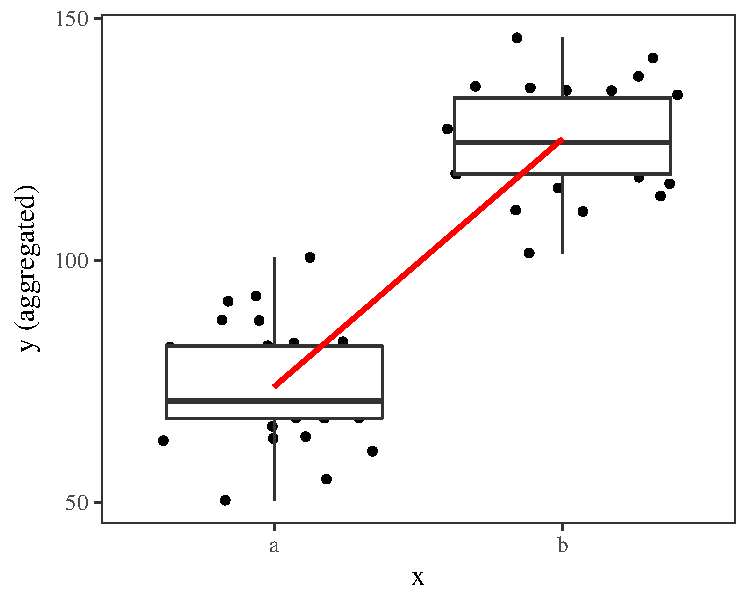
\includegraphics[scale = .6]{gfx/aggregateddatareg.pdf}
%		\caption{Simulated data, aggregated by subject and condition}
%		\end{figure}		
%\end{frame}



\begin{frame}
	\frametitle{Linear mixed effects models}
		
		\only<1>{
		\begin{figure}
			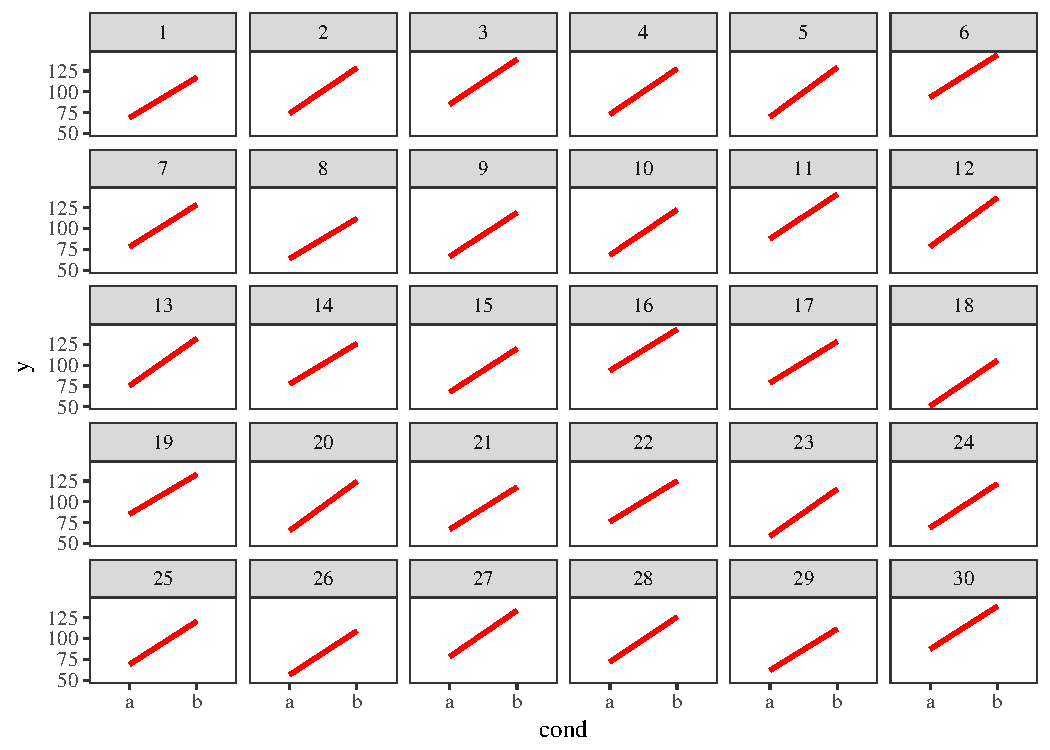
\includegraphics[scale = .5]{gfx/varyingintercepts.pdf}
			\caption{Varying intercepts per subject: $(1|subj)$}
		\end{figure}
	}
		\only<2>{
		\begin{figure}
			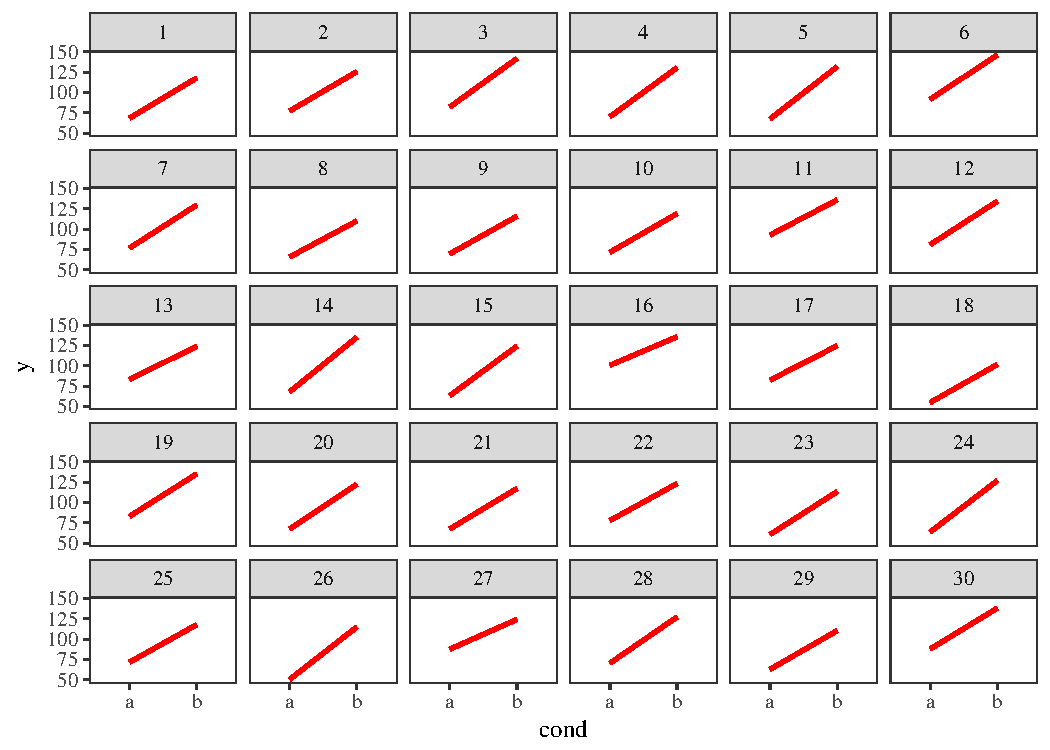
\includegraphics[scale = .5]{gfx/varyingeffects.pdf}
			\caption{Varying intercepts and slopes per subject: $(1+cond|subj)$}
		\end{figure}
	}
	
\end{frame}


\begin{frame}
	\frametitle{Linear mixed effects models}
	% p-values
	\begin{itemize}
		\item What about \textit{p}?
		\item Unclear how to determine df \cite<see>{baa08book}
		\item Alternatives:
		\begin{itemize}
			\item \textit{t}-value $=2$ as lower bound for $p < 0.05$
			\item Satterthwaite approximation $lmerTest$ package
			\item Model comparison using log likelihood ratio $anova()$
			
		\end{itemize}
		\item See $LMER\_pvalues.R$
	\end{itemize}	
	
\end{frame}

\begin{frame}
	\frametitle{Linear mixed effects models}
% a significant effect is not interesting if the effect magnitude is too small to be interesting
	\begin{itemize}
		\item \textit{p}-values do \textbf{not} tell us whether the difference is large enough to reject the null.
		\item This relies on the variance within each condition.
		
		\item We may reject the null for estimates that are too small to be sensible (e.g. $\sim 5ms$) if the variance is small enough
		
		\item \dots or fail to reject the null for sensible estimates that if the variance is too large.
		
%		\item Probability of observing a test statistic (t-value, F-ratio) at least as extreme if the null were true  

		\item It's not about a single value but a range.
		\item Is $0$ a possible value?
	\end{itemize}	
	
\end{frame}


\begin{frame}
	\frametitle{Linear mixed effects models}
	\begin{itemize}
%		\item Range of possible values of the effect in the population 
		\item 95\% confidence intervals (CI): 
		\item[] If we were to repeat our experiment an infinite number of times and calculate a confidence interval each time, 95\% of these intervals would contain the true parameter value.
		\item See simulation: \url{http://rpsychologist.com/d3/CI/}
		\item In other words, the estimate is merely the centre of a range of a imaginary range of other intervals which contains the population parameter.
		\item 5\% of these unobserved ranges do not contain the true value. 
		\item See exercises script $LMER95\%CIs.R$
	\end{itemize}

\end{frame}


\begin{frame}
	\frametitle{Linear mixed effects models}
	
	Advantages:
	\begin{itemize}
		\item Flexible models that account for the complexity of data
		\item Nested data: children nested in classes nested in schools %nested in cities etcetera
		\item Random effects: subject speed varies; effect varies across individuals; slopes and intercepts are correlated
		\item For a short but thorough intro see \citeA{vasishth2016statistical}
		 
	\end{itemize}
	
\end{frame}		


\begin{frame}
	\frametitle{Linear mixed effects models}
	
	Problem:
	\begin{itemize}

		\item Maximal random effects structure \cite{barr2013random}:\\ $(1+cond|subject) + (1+cond|item)$
		\only<1>{
		\item Random effects can be added: 
		\item[i.] $(1+cond|subject)$ accounts for varying conditional differences across subjects; not plausible in a between subjects design
		\item[ii.] $(1+cond|items)$ accounts for varying conditional differences across items; effect is stronger in some items %stress-shift in two words that identical on the surface, e.g., recOrd vs.~rEcord
		\item[] Not plausible when there were no matched items 
		}
		\only<2>{  
		\item Convergence failure: over-parametrisation \cite{bates2015parsimonious}:
		\item[] I.e. model is too complex for the data.
		\item Solution (i): remove random slopes until model converges
		\item Solution (ii): Bayesian Linear Mixed Effects Models 
		}
	\end{itemize}
	
\end{frame}	